\section{对偶问题与解的证书}
\label{sec:opt-lp-duality}

单纯形法报告“$(4/3,4/3)$最优，获利$20/3$”。别人若不想重跑算法，怎样确认这句话？验证可行性很容易，代入约束即可；难的是确认没有更好的产量。本节从“给获利找一个上界”出发，把约束按非负权重相加，得到线性规划的对偶问题。原问题和对偶问题互相给出界，二者同值时就证明了最优；单纯形法停止时的乘子$\bm y$恰好就是这样一组权重。同样的思路还为“不可行”和“无下界”分别给出可以核对的证据。

\subsection{对偶的构造与弱对偶}
\label{sec:opt-lp-weak-duality}

\paragraph{把约束加起来}
在资源模型~\eqref{eq:opt-lp-resource}中，把第一条原料约束乘以$u_1\ge0$，第二条乘以$u_2\ge0$，相加得
\[
  (2u_1+u_2)x_1+(u_1+2u_2)x_2\le4u_1+4u_2.
\]
若权重满足$2u_1+u_2\ge3$与$u_1+2u_2\ge2$，则由$x_1,x_2\ge0$，左边不小于获利$3x_1+2x_2$，于是任何可行产量的获利都不超过$4u_1+4u_2$。例如$\bm u=(1,1)$给出上界$8$，$\bm u=(2,1)$给出上界$10$，$\bm u=(4/3,1/3)$给出上界$20/3$。最后一个上界恰好等于$(4/3,4/3)$的获利，所以不可能有更好的产量。这一行推导不依赖任何算法，任何人都能复核。

权重可以解释为原料的价格。设想有人想把作坊的全部原料买下，给两种原料分别出价$u_1,u_2$。作坊只有在“把做一件产品所需的原料卖掉”至少不比“做成产品卖掉”少赚时才愿意出售，即$2u_1+u_2\ge3$、$u_1+2u_2\ge2$；买方则希望总价$4u_1+4u_2$尽量低。买方的问题
\begin{equation}
\label{eq:opt-lp-resource-dual}
  \min_{u_1,u_2}\ 4u_1+4u_2
  \quad\text{s.t.}\quad
  2u_1+u_2\ge3,\quad u_1+2u_2\ge2,\quad u_1,u_2\ge0
\end{equation}
就是在寻找最紧的上界。图~\ref{fig:opt-lp-dual-bounds}(a)画出了价格的可行域，它在$(4/3,1/3)$处取得最小总价$20/3$。

\begin{figure*}[!htbp]
  \centering
  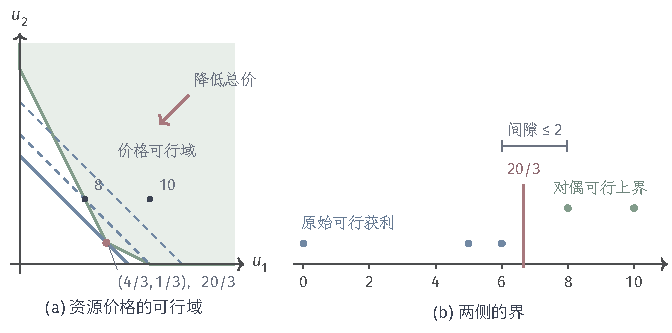
\includegraphics[width=113.771mm]{figures/03-optimization-evolution-and-signals/01-optimization/tikz/c2-dual-bounds/figure.pdf}
  \caption{原料价格给出的上界。(a) 绿色区域是满足式~\eqref{eq:opt-lp-resource-dual}约束的价格$(u_1,u_2)$，蓝色线是总价$4u_1+4u_2$的等值线，实线为最小总价$20/3$，在红点$(4/3,1/3)$处取得；黑点$(1,1)$与$(2,1)$也可行，总价为$8$和$10$。(b) 数轴上，蓝点是可行产量$(0,0)$、$(1,1)$、$(2,0)$的获利$0,5,6$，绿点是可行价格的总价$8,10$。每个蓝点都在每个绿点左侧；最优获利与最小总价都在$20/3$处，由$6$与$8$已能确定最优值落在长度为$2$的区间内。}
  \label{fig:opt-lp-dual-bounds}
\end{figure*}

\paragraph{标准型的对偶问题}
对标准型~\eqref{eq:opt-lp-standard}做同样的事。约束是等式，任意符号的权重都不改变等号方向，所以给第$i$个等式配一个可正可负的权重$y_i$。若$\bm A^\top\bm y\le\bm c$，则对任意可行$\bm x$，
\[
  \bm b^\top\bm y=(\bm A\bm x)^\top\bm y=\bm x^\top(\bm A^\top\bm y)\le\bm x^\top\bm c,
\]
不等号用到了$\bm x\ge\bm 0$：对非负的$x_j$，把系数$(\bm A^\top\bm y)_j$放大为$c_j$只会使乘积变大。于是每个满足$\bm A^\top\bm y\le\bm c$的$\bm y$都给出原问题最优值的一个下界$\bm b^\top\bm y$，最好的下界由下面的问题给出。

\begin{definition}[线性规划的对偶问题]
\label{def:opt-lp-dual}
标准型~\eqref{eq:opt-lp-standard}的\term{对偶问题}（dual problem）是
\begin{equation}
\label{eq:opt-lp-dual}
  \max_{\bm y\in\mathbb R^m}\ \bm b^\top\bm y
  \quad\text{s.t.}\quad
  \bm A^\top\bm y\le\bm c.
\end{equation}
相对地，称式~\eqref{eq:opt-lp-standard}为\term{原始问题}（primal problem）。满足对偶约束的$\bm y$称为对偶可行。
\end{definition}

\begin{theorem}[弱对偶]
\label{thm:opt-lp-weak-duality}
若$\bm x$对原始问题可行、$\bm y$对对偶问题可行，则$\bm b^\top\bm y\le\bm c^\top\bm x$。特别地，若二者相等，则$\bm x$与$\bm y$分别是两个问题的最优解。
\end{theorem}

上面的推导就是证明。第二句成立是因为：任何其他原始可行点的目标值都不小于$\bm b^\top\bm y=\bm c^\top\bm x$，任何其他对偶可行点的目标值都不大于$\bm c^\top\bm x=\bm b^\top\bm y$。这就是\term{弱对偶}（weak duality）。差$\bm c^\top\bm x-\bm b^\top\bm y\ge0$称为这对可行点的\term{对偶间隙}（duality gap），它同时控制了两侧离最优值有多远：$\bm c^\top\bm x-f^\star\le\bm c^\top\bm x-\bm b^\top\bm y$。间隙为零就证明了最优，而且只需要核对两组可行性和两个数是否相等，不需要第~\ref{chap:constrained-optimization}章的一般KKT理论。

\paragraph{符号规则来自同一个推导}
不同形式的原始约束对应不同的对偶符号，但不必死记表格：每次都回到“加权相加后仍保持不等号方向”这一推导即可。以资源模型为例，它是最大化问题，约束取“$\le$”，可行的获利是最优值的下界；要得到上界，“$\le$”约束的权重必须非负，否则乘以负数会把不等号反向，这就是$u_1,u_2\ge0$的来历；变量非负，所以只需权重组合后的系数“盖住”获利系数，得到$\ge$型的对偶约束。把资源模型写成例~\ref{ex:opt-lp-resource-standard}的标准型再套用式~\eqref{eq:opt-lp-dual}，对偶约束为$2y_1+y_2\le-3$、$y_1+2y_2\le-2$、$y_1\le0$、$y_2\le0$（后两条来自松弛变量的列），令$\bm u=-\bm y$即得式~\eqref{eq:opt-lp-resource-dual}，两种写法一致。最小化问题中原始值在上、对偶值在下；最大化问题中方向相反。图~\ref{fig:opt-lp-dual-bounds}(b)把最大化例子中两侧的界画在同一条数轴上。

\subsection{强对偶与互补松弛}
\label{sec:opt-lp-strong-duality}

弱对偶只说明下界不超过上界。我们关心的是：最好的下界是否恰好等于最优值？对线性规划，单纯形法的终止状态直接给出肯定的回答。

\begin{theorem}[线性规划强对偶]
\label{thm:opt-lp-strong-duality}
若标准型~\eqref{eq:opt-lp-standard}可行且目标在可行域上有下界，则原始问题与对偶问题~\eqref{eq:opt-lp-dual}都有最优解，并且两个最优值相等。
\end{theorem}

\begin{proof}
先把$\bm A$化为满行秩。原问题可行，等式系统相容；删去冗余行后得到$\bm A'\bm x=\bm b'$，可行域不变。若$\bm y'$对删行后的问题对偶可行，把删去的行对应的分量补为零得到$\bm y$，则$\bm A^\top\bm y=\bm A'^\top\bm y'$、$\bm b^\top\bm y=\bm b'^\top\bm y'$，所以对偶可行性和对偶目标值都不变。下面设$\bm A$满行秩。

对原问题执行两阶段法，两个阶段都使用Bland规则。由定理~\ref{thm:opt-lp-phase-one}与定理~\ref{thm:opt-lp-finite}，第一阶段在有限步后停止，最优值为零（原问题可行），把人工变量换出基后得到可行基。第二阶段同样在有限步后停止；由于目标有下界，不会以无下界方向结束，所以停在满足$\bar{\bm c}_N\ge\bm 0$的基$B$上，基本可行解记为$\bm x^\star$。

令$\bm y^\star=\bm A_B^{-\top}\bm c_B$。约化费用$\bar{\bm c}=\bm c-\bm A^\top\bm y^\star$在基指标上为零，在非基指标上非负，所以$\bm A^\top\bm y^\star\le\bm c$，$\bm y^\star$对偶可行。又
\[
  \bm b^\top\bm y^\star=\bm b^\top\bm A_B^{-\top}\bm c_B=\bm c_B^\top\bm A_B^{-1}\bm b=\bm c_B^\top\bm x^\star_B=\bm c^\top\bm x^\star.
\]
由弱对偶，$\bm x^\star$与$\bm y^\star$分别最优，且最优值相等。
\end{proof}

原始与对偶最优值相等的结论称为\term{强对偶}（strong duality）。证明说明了单纯形法中乘子$\bm y$的身份：它就是对偶最优解，而“约化费用全部非负”与“$\bm y$对偶可行”是同一件事。在资源模型中，表~\ref{tab:opt-lp-simplex-run}最后一轮的$\bm y=(-4/3,-1/3)^\top$，对应价格$\bm u=-\bm y=(4/3,1/3)$，正是图~\ref{fig:opt-lp-dual-bounds}(a)的最优价格。这一强对偶结论只要求原问题可行、有下界，不需要任何内点条件；第~\ref{chap:constrained-optimization}章讨论一般凸问题时，零间隙要借助Slater条件之类的额外假设，那是线性结构以外才需要的。

\paragraph{互补松弛}
对一对可行点，把间隙展开：
\[
  \bm c^\top\bm x-\bm b^\top\bm y=\bm c^\top\bm x-(\bm A\bm x)^\top\bm y=\bm x^\top(\bm c-\bm A^\top\bm y)=\sum_{j=1}^nx_j\,(c_j-\bm a_j^\top\bm y).
\]
求和中的每一项都是两个非负数的乘积，所以间隙为零当且仅当每一项都为零。

\begin{theorem}[互补松弛]
\label{thm:opt-lp-complementary-slackness}
设$\bm x$原始可行、$\bm y$对偶可行。二者同为最优解，当且仅当对每个$j$，
\[
  x_j\,(c_j-\bm a_j^\top\bm y)=0,
\]
即$x_j>0$时第$j$条对偶约束取等号，第$j$条对偶约束严格成立时$x_j=0$。
\end{theorem}

\begin{proof}
若二者都最优，由定理~\ref{thm:opt-lp-strong-duality}，两侧最优值相等（原问题有可行点，又有对偶可行点给出下界），间隙为零，各项均为零。反之各项为零时间隙为零，由弱对偶二者最优。
\end{proof}

这一条件称为\term{互补松弛}（complementary slackness）。在资源模型中，$\bm x^\star=(4/3,4/3,0,0)^\top$，$\bm c-\bm A^\top\bm y^\star=(0,0,4/3,1/3)^\top$，逐项乘积全为零，两侧值都是$-20/3$（最大化写法中都是$20/3$）。翻译回资源语言：两种产品都在生产（$x_1,x_2>0$），所以每件产品的获利恰好等于它消耗的原料按价格折算的价值，$2\cdot\frac43+\frac13=3$、$\frac43+2\cdot\frac13=2$；两种原料都有正价格，所以它们都被用完（松弛变量$x_3=x_4=0$）。反过来，有剩余的原料价格必为零：多出来的原料不值钱。

\paragraph{最优面是一个面}
互补松弛还说明了第~\ref{sec:opt-lp-polyhedra}节中“最优面”这一名称的来由。取定一个对偶最优解$\bm y^\star$，可行点$\bm x$最优当且仅当$x_j=0$对每个满足$c_j-\bm a_j^\top\bm y^\star>0$的$j$成立。所以标准型的全部最优解恰好是让这些非负约束同时取等号所得的面。在图~\ref{fig:opt-lp-optimal-face}(b)中，最优价格只让第一种原料的松弛变量必须为零，最优面就是$x_3=0$那条边。

\paragraph{有限精度下怎样报告}
数值求解器给出的$\bm x$与$\bm y$通常各自只近似可行。此时应同时报告四个量：原始等式残差$\lVert\bm A\bm x-\bm b\rVert$、原始变量的负部、对偶约束的违反量$\max_j\max\{\bm a_j^\top\bm y-c_j,0\}$，以及间隙$\bm c^\top\bm x-\bm b^\top\bm y$。只有在$\bm y$确实对偶可行时，$\bm b^\top\bm y$才是合法的下界；只有在$\bm x$确实可行时，$\bm c^\top\bm x$才是可以达到的值。不满足可行性的两个数之差不能直接当作误差上界。例如资源模型中取价格$\bm u=(1.4,0.2)$，它满足$2u_1+u_2\ge3$，却违反$u_1+2u_2\ge2$（左边为$1.8$）；它给出的“上界”$4u_1+4u_2=6.4$小于真实最优值$20/3$。若忽略这一点违反，就会错误地断言获利不可能超过$6.4$。

\subsection{不可行与无下界的证书}
\label{sec:opt-lp-certificates}

线性规划只有三种结局：有最优解、不可行、可行但无下界。前一小节为第一种结局给出了证书：一对原始、对偶可行点，间隙为零。另外两种结局也有类似的、可以独立核对的证据。

\paragraph{不可行的证书}
若再要求两种产品合计至少生产$5$件，资源模型就不可行。证据是什么？把两条原料约束各乘$1/3$相加，得到$x_1+x_2\le8/3$，与$x_1+x_2\ge5$矛盾。一般地，不可行性可以由一组权重这样“组合出矛盾”来证明，而且只要不可行，这样的权重一定存在。

\begin{theorem}[Farkas择一定理]
\label{thm:opt-lp-farkas}
给定$\bm A\in\mathbb R^{m\times n}$与$\bm b\in\mathbb R^m$，下面两个系统恰有一个有解：
\[
  \text{（甲）}\ \bm A\bm x=\bm b,\ \bm x\ge\bm 0;
  \qquad
  \text{（乙）}\ \bm A^\top\bm z\ge\bm 0,\ \bm b^\top\bm z<0.
\]
\end{theorem}

\begin{proof}
二者不能同时有解：否则$0>\bm b^\top\bm z=\bm x^\top\bm A^\top\bm z\ge0$，矛盾。

再设（甲）无解，构造（乙）的解。先把$b_i<0$的行乘以$-1$：记$\bm D$为对角元是$\pm1$的对角矩阵，使$\widetilde{\bm A}=\bm D\bm A$、$\widetilde{\bm b}=\bm D\bm b\ge\bm 0$。对$\widetilde{\bm A},\widetilde{\bm b}$构造第一阶段问题~\eqref{eq:opt-lp-phase-one}，按Bland规则求解。由定理~\ref{thm:opt-lp-finite}，它在有限步后停在一个最优基上，乘子记为$\bm w$，约化费用全部非负。原变量$x_j$的费用为$0$，所以$0-\widetilde{\bm a}_j^\top\bm w\ge0$，即$\widetilde{\bm A}^\top\bm w\le\bm 0$。最优值等于$\widetilde{\bm b}^\top\bm w$（与强对偶证明中的计算相同），由定理~\ref{thm:opt-lp-phase-one}和（甲）无解，它严格为正。令$\bm z=-\bm D\bm w$，则
\[
  \bm A^\top\bm z=-\bm A^\top\bm D\bm w=-\widetilde{\bm A}^\top\bm w\ge\bm 0,\qquad
  \bm b^\top\bm z=-\widetilde{\bm b}^\top\bm w<0.
\]
\end{proof}

满足（乙）的$\bm z$称为（甲）的不可行证书，这一结论通常称为\term{Farkas引理}（Farkas lemma）。核对它只需一次矩阵乘法：若有可行$\bm x$，则$\bm z^\top\bm b=\bm z^\top\bm A\bm x$是非负数$(\bm A^\top\bm z)_j$与非负数$x_j$乘积之和，不可能为负。证明的后半部分不是抽象的存在性论证：它说明第一阶段停止时的乘子$\bm w$取负号就是证书，求解器判定不可行时可以把它一并输出。

\begin{example}[合计至少五件]
\label{ex:opt-lp-farkas}
标准型变量为$x_1,\dots,x_5$，约束为$2x_1+x_2+x_3=4$、$x_1+2x_2+x_4=4$、$x_1+x_2-x_5=5$。第一阶段只需为第三行加人工变量。依Bland规则，$x_1$入基、$x_3$出基，再$x_2$入基、$x_4$出基，停在基$\{x_1,x_2,a\}$上，此时$x_1=x_2=4/3$，人工变量$a=7/3$，最优值$7/3>0$，乘子$\bm w=(-1/3,-1/3,1)^\top$。取$\bm z=-\bm w=(1/3,1/3,-1)^\top$，逐列核对$\bm A^\top\bm z$：$x_1$列$\tfrac23+\tfrac13-1=0$，$x_2$列$\tfrac13+\tfrac23-1=0$，$x_3,x_4,x_5$列分别为$\tfrac13,\tfrac13,1$，全部非负；而$\bm b^\top\bm z=\tfrac43+\tfrac43-5=-\tfrac73<0$。这组权重正是开头那句推理：两条原料约束各取$1/3$，再与产量要求相减。
\end{example}

图~\ref{fig:opt-lp-farkas}给出了定理的几何含义。$\{\bm A\bm x:\bm x\ge\bm 0\}$是$\bm A$的各列张成的锥$K$，（甲）有解就是$\bm b\in K$。当$\bm b$在锥外时，存在一个过原点的超平面$\{\bm v:\bm z^\top\bm v=0\}$，把整个锥留在$\bm z^\top\bm v\ge0$一侧，把$\bm b$放在另一侧；（乙）的两个条件说的正是这件事。

\begin{figure}[!htbp]
  \centering
  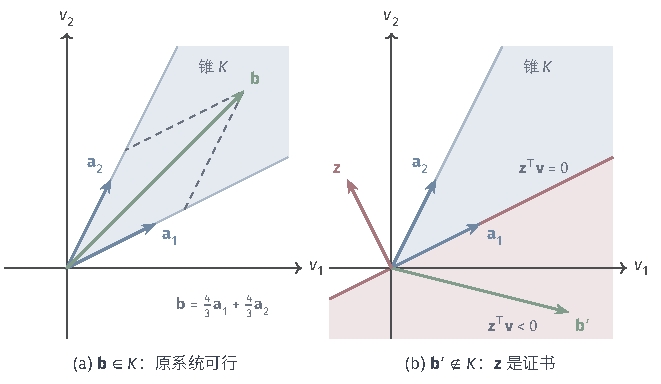
\includegraphics[width=111.898mm]{figures/03-optimization-evolution-and-signals/01-optimization/tikz/c2-farkas/figure.pdf}
  \caption{Farkas择一定理的几何。两列$\bm a_1=(2,1)$、$\bm a_2=(1,2)$张成锥$K$（浅蓝）。(a) $\bm b=(4,4)=\tfrac43\bm a_1+\tfrac43\bm a_2$在锥内，系统$\bm A\bm x=\bm b$、$\bm x\ge\bm 0$有解。(b) $\bm b'=(4,-1)$在锥外；$\bm z=(-1,2)$满足$\bm a_1^\top\bm z=0$、$\bm a_2^\top\bm z=3$、$\bm b'^\top\bm z=-6$，红线$\bm z^\top\bm v=0$把锥与$\bm b'$分在两侧，浅红半平面是$\bm z^\top\bm v<0$的一侧。}
  \label{fig:opt-lp-farkas}
\end{figure}

\paragraph{无下界的证书}
若原问题可行但无下界，证据是一个已知的可行点$\bm x_0$加一个方向$\bm d$，满足
\[
  \bm A\bm d=\bm 0,\qquad\bm d\ge\bm 0,\qquad\bm c^\top\bm d<0.
\]
核对很直接：对任意$t\ge0$，$\bm x_0+t\bm d$可行，目标$\bm c^\top\bm x_0+t\bm c^\top\bm d\to-\infty$。单纯形法在比值检验中发现$\bm d_B\ge\bm 0$时，返回的正是这样一对$(\bm x,\bm d)$。图~\ref{fig:opt-lp-polyhedron-cases}(c)是一个例子：标准型为$\min\ x_2-x_1$，约束$x_1+x_2-x_3=1$，$\bm x\ge\bm 0$；取$\bm x_0=(1,0,0)^\top$、$\bm d=(1,0,1)^\top$，有$\bm A\bm d=1+0-1=0$，$\bm c^\top\bm d=-1<0$。

\paragraph{三种不可行要分开}
原问题不可行、原问题无下界与对偶问题不可行是三件不同的事，它们之间只有部分蕴含关系。由弱对偶，原问题无下界时不可能有对偶可行点，否则它会给出有限下界，所以对偶问题不可行；上面的例子中对偶约束为$y\le-1$、$y\le1$、$-y\le0$，确实无解。反方向需要额外条件：只有在已经知道原问题可行时，才能由对偶不可行推出原问题无下界，因为若原问题可行且有下界，定理~\ref{thm:opt-lp-strong-duality}会给出对偶最优解。若不知道原问题是否可行，这一推理不成立。例如
\[
  \min\ -x_1-x_2\quad\text{s.t.}\quad x_1-x_2=1,\quad -x_1+x_2=1,\quad\bm x\ge\bm 0
\]
的两个等式相加得$0=2$，原问题不可行；它的对偶约束$y_1-y_2\le-1$与$-y_1+y_2\le-1$相加得$0\le-2$，对偶问题也不可行。方向$\bm d=(1,1)^\top$满足$\bm A\bm d=\bm 0$、$\bm d\ge\bm 0$、$\bm c^\top\bm d=-2<0$，可是没有可行的起点，它不能说明任何东西“无下界”。所以报告无下界时，必须同时给出可行点和方向，二者缺一不可。
